\subsection{问题三求解思路}

问题三在场景 B 的基础上增加一块所有核心共享的只读 L2 Cache，容量 $C_{L2}=1{,}048{,}576$ 字节，带宽 $B_{L2}=250$ bytes/cycle，与 DDR 带宽相互独立。根据题目附录 D.5 与评估程序的实现，它的规则可以归纳为四条：只有 COPY\_IN 查询缓存，COPY\_OUT 总是写 DDR，查询发生在 COPY\_IN 发射时刻，键为逻辑张量编号，同一张量被不同核心读取时键相同；命中的 COPY\_IN 进入缓存带宽池，多个命中公平共享 250 bytes/cycle，不占 DDR 带宽，未命中的走 DDR；未命中的 COPY\_IN 完成后才把张量写入缓存，容量不足时按先进先出淘汰，命中不改变淘汰顺序，大于容量的张量不缓存；命中率按字节计。

这几条规则决定了求解思路。命中需要同一张量此前已被读过、那次读取已经完成、并且之后写入的数据还没把它挤出去，这是时序条件和容量条件；命中省下的是 DDR 带宽，只有 DDR 确实繁忙时才能换来时间。所以我们先写出缓存状态的演化和命中的充要条件，据此把未命中分类，再用 DDR 忙碌占比刻画命中能换来多少时间，并给出缓存加速比的带宽上限。求解上，问题三与问题二同属场景 B，方案可以互换，问题二的全部候选都交给问题三的评估程序复评，再在缓存评估下做后处理。题目要求研究的容量和带宽影响，通过固定一批方案、只改缓存参数重新评估来回答。

\subsection{问题三模型建立}\label{sec:p3-math}

\subsubsection{缓存状态与命中条件}

把缓存内容记为按写入先后排列的队列 $\mathcal{Q}(\tau)=(t_1,t_2,\dots)$，占用 $|\mathcal{Q}|=\sum_{t\in\mathcal{Q}}s_t$。一次未命中的 COPY\_IN 在完成时刻写入张量 $t$（若 $s_t\le C_{L2}$ 且 $t\notin\mathcal{Q}$），写入前先从队首淘汰，直到放得下：
\begin{equation}
  \text{while }\ |\mathcal{Q}|+s_t>C_{L2}:\ \ \mathcal{Q}\leftarrow\mathcal{Q}\setminus\{\text{队首}\};\qquad \mathcal{Q}\leftarrow\mathcal{Q}\oplus t .
  \label{eq:fifo}
\end{equation}
命中的读取与 DDR 读取分别在两个独立的带宽池中按式 \eqref{eq:fair-share} 的方式公平共享：
\begin{equation}
  \frac{\mathrm{d}w_j}{\mathrm{d}\tau}=
  \begin{cases}
  -B_{L2}/m_{L2}(\tau), & j\ \text{命中},\\
  -B/m_{\mathrm{DDR}}(\tau), & j\ \text{未命中或为 COPY\_OUT},
  \end{cases}
  \label{eq:pools}
\end{equation}
即命中的读取只和其他命中读取分享 $B_{L2}$，不占用 DDR；未命中的读取和全部写出仍在 DDR 池中分享 $B$。命中越多，DDR 池中的 $m_{\mathrm{DDR}}(\tau)$ 越小，其余搬运分到的带宽就越大，这是缓存能缩短 Makespan 的途径。字节命中率为
\begin{equation}
  \theta=\frac{\sum_{j\ \text{命中}} s_j}{\sum_{j\ \text{为 COPY\_IN}} s_j}.
  \label{eq:hitrate}
\end{equation}

记第 $j$ 次 COPY\_IN 读取的逻辑张量为 $t_j$，发射、完成时刻为 $a_j,e_j$。它命中当且仅当存在更早的一次未命中读取 $i$（$t_i=t_j$），满足
\begin{equation}
  e_i\le a_j\qquad\text{且}\qquad \sum_{\ell\in\mathcal{I}(e_i,a_j)} s_\ell\ \le\ C_{L2}-s_{t_j},
  \label{eq:hit}
\end{equation}
$\mathcal{I}(e_i,a_j)$ 为在 $(e_i,a_j]$ 内写入缓存的其他张量。第一式是时序条件：张量在未命中读取完成时才写入缓存，而查询发生在发射时刻，所以只有 $e_i\le a_j$ 时第 $j$ 次查询才可能看到它。第二式是容量条件：由式 \eqref{eq:fifo}，张量写入后只会因后来写入的数据而被挤出，命中又不改变队列顺序，只要其后写入的总字节数不超过 $C_{L2}-s_{t_j}$，它就仍在队列中。两个条件同时成立时查询必然命中；反过来，命中的张量一定是某次未命中读取写入且尚未淘汰的，两个条件都成立，所以式 \eqref{eq:hit} 是充要条件。据此把每次未命中分为三类\cite{hill1989evaluating}：
\begin{equation}
  \text{缺失类型}(j)=
  \begin{cases}
  \text{首次缺失}, & \text{此前没有任何读取 } i<j,\ t_i=t_j;\\
  \text{并发缺失}, & \text{存在 } i<j,\ t_i=t_j,\ \text{但所有这样的 } i \text{ 都有 } e_i>a_j;\\
  \text{容量缺失}, & \text{曾经写入，但已被先进先出淘汰。}
  \end{cases}
  \label{eq:miss-class}
\end{equation}
首次缺失由计算图决定，任何调度都消除不了；容量缺失与缓存大小和写入次序有关；并发缺失则完全是时序问题：多个核心几乎同时读同一个张量，第一次读取还没完成，其余读取全部落空，同时挤占 DDR。

\subsubsection{缓存收益与带宽上限}\label{sec:p3-benefit}

一次命中节省的 DDR 占用为 $s_j/B$ 周期，但能否转化为 Makespan 的缩短，取决于 DDR 是不是瓶颈。定义无 L2 时的 DDR 忙碌占比与同一方案的缓存加速比
\begin{equation}
  \beta=\frac{Q_{\mathrm{DDR}}}{B\cdot M^{\mathrm{noL2}}},\qquad
  \gamma=\frac{M^{\mathrm{noL2}}}{M^{\mathrm{cache}}},
  \label{eq:ddr-busy}
\end{equation}
$Q_{\mathrm{DDR}}$ 为全部 DDR 搬运字节数。$\beta$ 很小时 DDR 大部分时间空闲，省下的带宽没有别的搬运去用，命中只让个别 COPY\_IN 快一点，未必落在关键路径上；$\beta$ 接近 1 时，命中直接减轻了争用，所有在途搬运都会变快。所以 $\gamma$ 应随 $\beta$ 上升。进一步，记只读 Cache 配置下仍走 DDR 的字节数为 $Q_D$、命中字节数为 $Q_H$，无 L2 时这些字节全部走 DDR。只读 Cache 下 $M^{\mathrm{cache}}\ge Q_D/B$；若无 L2 时 Makespan 完全由 DDR 带宽决定，即 $M^{\mathrm{noL2}}\approx (Q_D+Q_H)/B$，则
\begin{equation}
  \gamma=\frac{M^{\mathrm{noL2}}}{M^{\mathrm{cache}}}\ \le\ \frac{(Q_D+Q_H)/B}{Q_D/B}=\bar\gamma=1+\frac{Q_H}{Q_D}.
  \label{eq:gamma-bound}
\end{equation}
式 \eqref{eq:gamma-bound} 是带宽完全饱和这一理想情形下的上限，前提不总成立，因此只作估计。缓存也可能让同一方案变慢：命中改变了 COPY\_IN 的完成时刻，而核内操作顺序是固定的，完成时刻的变化可能让关键路径上的某个操作等待更久，这是多处理机调度中已知的时序异常\cite{graham1969bounds}。

\subsubsection{问题三的优化模型}

问题三的决策变量与约束与问题二相同，目标由问题三的评估程序给出：
\begin{equation}
\begin{aligned}
  \min\quad & M_k^{\mathrm{cache}}=\max_{v\in\Oe} f_v\\
  \text{s.t.}\quad & \text{问题二的全部约束 \eqref{eq:assign}--\eqref{eq:order}、\eqref{eq:sync-B}--\eqref{eq:resident}},\\
  & \text{COPY\_IN 按命中条件 \eqref{eq:hit} 选择带宽池 \eqref{eq:pools}，缓存内容按式 \eqref{eq:fifo} 更新},
\end{aligned}
  \label{eq:obj-p3}
\end{equation}
并以同核数下两种配置各自最优方案的缓存加速比
\begin{equation}
  \Gamma_k=\frac{M_k^{\mathrm{noL2,*}}}{M_k^{\mathrm{cache,*}}}
  \label{eq:Gamma}
\end{equation}
作为题目要求报告的指标。由式 \eqref{eq:hit}--\eqref{eq:gamma-bound}，好的问题三方案要同时满足三点：DDR 足够紧张，缓存才有意义；共享同一输入的消费者分散在几个核心上，缓存才有重复读取可以服务；这些读取在时间上错开，命中条件才能成立。前两点会增加跨核依赖，第三点要求读取有先后，三者之间存在张力。

\subsection{问题三模型求解与结果分析}

\subsubsection{算法描述}\label{sec:p3-solve}

问题三的候选池包括问题二的全部候选方案，再加上在问题三评估程序下做的后处理，流程仍为算法~\ref{alg:select}，只是把 $E_p$ 换成问题三的评估程序。第一步是交叉复评。这一步的起因是 case\_061 3 核：问题三原来的最优方案来自相位构造，Makespan 为 36{,}250；问题二中经成组合并（宽度 16、全部核心）得到的方案放到问题三评估程序下只有 28{,}368，缩短 21.7\%。只在本问题的最优起点上做后处理会漏解。因此我们把问题一、二、三各来源的获胜方案按内容哈希去重后，逐个交给问题二、三的评估程序，并在最终阶段把两问的最终方案再互相复评一次，使两种配置在“各自最优”口径下的候选池对称。

第二步是在缓存评估下重做成组合并与局部搜索。成组合并改变同核子图的执行顺序（第~\ref{sec:p2-coarsen} 节），也就改变了共享张量被读取的先后，有可能把并发缺失变成命中，所以在问题三评估程序下重新做一遍。局部搜索以问题三的 Makespan 为目标，优先用于缓存收益潜力大的用例。

另有两条针对缓存的路线在实验中被否定。一是在相位构造中加入缓存感知代价：某张量已被一个核心读过时，其他核心再读按缓存带宽计价，以鼓励把共享张量的消费者分散到多个核心。在第~\ref{sec:neg} 节的 12 个用例上，它相对问题三构造阶段选优的 Makespan 比值几何均值为 \V{neg_phasec_p3_d50000_geo}（$\lambda=5\times10^4$），没有一例更好。它鼓励跨核扇出，增加了跨核边和同步，而同时发起的读取按式 \eqref{eq:hit} 根本不会命中，按缓存带宽计价的前提本身不成立。二是错开读取的后处理：为每个共享张量指定一个领读核心，领读的子图排前、跟读的子图排后，只调整各核内子图的先后。它在并发缺失最多的用例上效果有限，因为锁步读取往往发生在同一条依赖链内部，调整子图顺序改变不了核间的相位差（实验记录见第~\ref{sec:neg-record} 节）。

\subsubsection{求解分析}

先检验缓存收益的影响因素。图~\ref{fig:ddr} 用 \V{fig_ddr_pairs} 组同方案配对检验了 $\gamma$ 与 $\beta$ 的关系：$\beta<20\%$ 时 $\gamma$ 平均只有 \V{fig_ddr_mean_0}，$\beta\ge 80\%$ 时达到 \V{fig_ddr_mean_4}。图~\ref{fig:cbound} 把最终方案（4 核）的实测 $\gamma$ 与上限 $\bar\gamma$ 放在一起：\V{figx_cb_n} 个用例中 \V{figx_cb_below} 个位于上限之下；按实际收益占上限收益的比例 $(\gamma-1)/(\bar\gamma-1)$ 计，$\beta\ge 60\%$ 的用例中位数为 \V{figx_cb_ratio_hi}，$\beta<30\%$ 的用例中位数为 \V{figx_cb_ratio_lo}。命中字节即使不少，DDR 不紧张时也几乎换不来时间。缓存让同一方案变慢的情况在全部 500 组同方案配对中出现了 \V{p3_same_worse_total} 次，最小比值为 \V{p3_same_min}。

\begin{figure}[H]
  \centering
  \begin{minipage}[t]{0.44\textwidth}
    \centering
    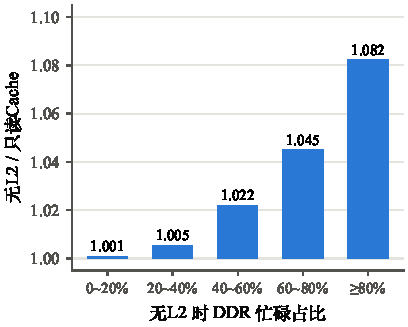
\includegraphics[width=\textwidth]{cache_vs_ddr}
    \caption{同一方案的缓存加速比与无 L2 时 DDR 忙碌占比}
    \label{fig:ddr}
  \end{minipage}\hfill
  \begin{minipage}[t]{0.53\textwidth}
    \centering
    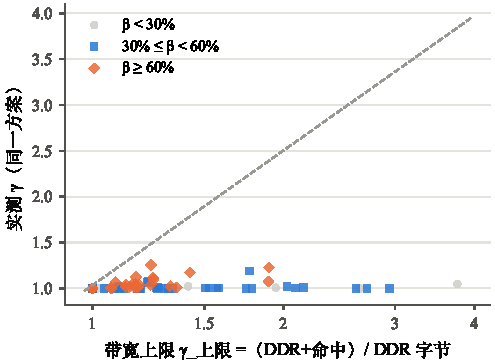
\includegraphics[width=\textwidth]{cache_bound}
    \caption{缓存加速比的实测值与带宽上限 $\bar\gamma$（4 核，最终方案；虚线为 $y=x$）}
    \label{fig:cbound}
  \end{minipage}
\end{figure}

用式 \eqref{eq:miss-class} 对最终方案（4 核）的全部缓存访问做分解（图~\ref{fig:miss}）。按字节计，命中占 \V{fig_miss_hit}，首次缺失占 \V{fig_miss_compulsory}，容量缺失 \V{fig_miss_capacity}，并发缺失 \V{fig_miss_concurrent}。三分之二左右的访问是首次读取，这是计算图决定的上限；在可以争取的部分中，并发缺失与容量缺失量级相当，所以问题三不能只从容量够不够来考虑。

\begin{figure}[H]
  \centering
  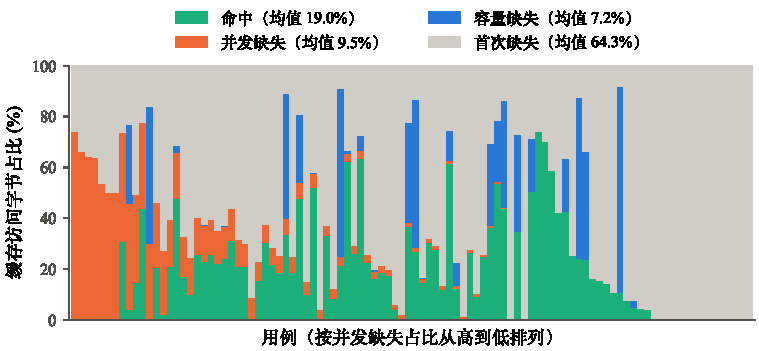
\includegraphics[width=\textwidth]{miss_breakdown}
  \caption{缓存访问的缺失分解（4 核，最终方案，按并发缺失占比从高到低排列）}
  \label{fig:miss}
\end{figure}

图~\ref{fig:p3} 给出 1--5 核下无 L2 与只读 Cache 两种配置的对比曲线和同核数下的缓存加速比，数值汇总在表~\ref{tab:p3-result}，逐用例的 Makespan、总额外搬运量和命中率见附录 C。5 核时只读 Cache 配置的平均加速比为 \V{p3_k5_cache_vs_single}，无 L2 为 \V{p3_k5_noL2_vs_single}；同核数下缓存加速比 $\Gamma_5$ 的均值为 \V{p3_k5_best_mean}，单个用例最高 \V{p3_k5_best_max}。缓存加速比随核数上升（1 核 \V{p3_k1_best_mean}，5 核 \V{p3_k5_best_mean}），命中率也从 \V{p3_k1_hit_mean} 升到 \V{p3_k5_hit_mean}：核数越多，同一张量被越多核心读取，DDR 越紧张，缓存越有用。快速模式下只用 9 个构造候选时，只读 Cache 配置 1--5 核的平均加速比为 \V{figx_fast_p3_k1_mean}、\V{figx_fast_p3_k2_mean}、\V{figx_fast_p3_k3_mean}、\V{figx_fast_p3_k4_mean}、\V{figx_fast_p3_k5_mean}，单个用例同样在数分钟内完成。

\begin{figure}[H]
  \centering
  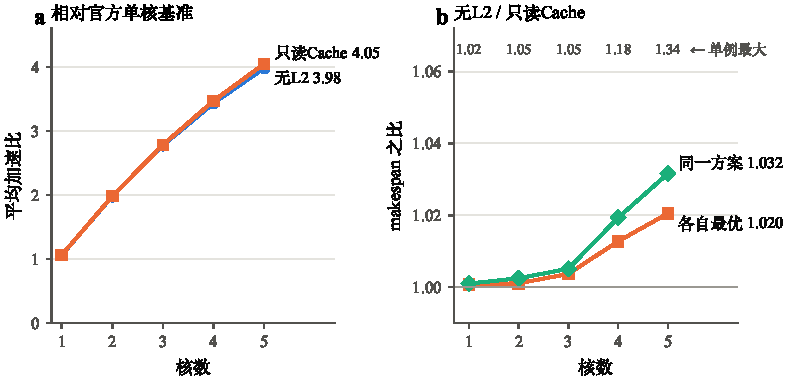
\includegraphics[width=\textwidth]{p3_compare}
  \caption{无 L2 与只读 Cache 两种配置的对比。(a) 两种配置各自逐用例选优后的平均加速比（相对官方单核基准）；(b) 同核数下只读 Cache 相对无 L2 的加速比，“各自最优”为两种配置分别取最优方案，“同一方案”为问题三所选方案放回无 L2 下复评；图顶数字为单例最大值}
  \label{fig:p3}
\end{figure}

\begin{table}[H]
\centering
\caption{问题三结果统计（100 个用例）}
\label{tab:p3-result}
\renewcommand\arraystretch{1.15}
\resizebox{\textwidth}{!}{%
\begin{tabular}{lccccc}
\toprule
 & 1 核 & 2 核 & 3 核 & 4 核 & 5 核 \\
\midrule
无 L2 平均加速比（相对单核基准） & \V{p3_k1_noL2_vs_single} & \V{p3_k2_noL2_vs_single} & \V{p3_k3_noL2_vs_single} & \V{p3_k4_noL2_vs_single} & \V{p3_k5_noL2_vs_single} \\
只读 Cache 平均加速比（相对单核基准） & \V{p3_k1_cache_vs_single} & \V{p3_k2_cache_vs_single} & \V{p3_k3_cache_vs_single} & \V{p3_k4_cache_vs_single} & \V{p3_k5_cache_vs_single} \\
\midrule
缓存加速比 $\Gamma_k$ 均值 & \V{p3_k1_best_mean} & \V{p3_k2_best_mean} & \V{p3_k3_best_mean} & \V{p3_k4_best_mean} & \V{p3_k5_best_mean} \\
\quad 单例最大 & \V{p3_k1_best_max} & \V{p3_k2_best_max} & \V{p3_k3_best_max} & \V{p3_k4_best_max} & \V{p3_k5_best_max} \\
\quad 提升超过 1\% / 5\% 的用例数 & \V{p3_k1_n_gain1pct} / \V{p3_k1_n_gain5pct} & \V{p3_k2_n_gain1pct} / \V{p3_k2_n_gain5pct} & \V{p3_k3_n_gain1pct} / \V{p3_k3_n_gain5pct} & \V{p3_k4_n_gain1pct} / \V{p3_k4_n_gain5pct} & \V{p3_k5_n_gain1pct} / \V{p3_k5_n_gain5pct} \\
同一方案的缓存加速比 $\gamma$ 均值 & \V{p3_k1_same_mean} & \V{p3_k2_same_mean} & \V{p3_k3_same_mean} & \V{p3_k4_same_mean} & \V{p3_k5_same_mean} \\
\midrule
平均命中率 $\theta$ & \V{p3_k1_hit_mean} & \V{p3_k2_hit_mean} & \V{p3_k3_hit_mean} & \V{p3_k4_hit_mean} & \V{p3_k5_hit_mean} \\
平均额外搬运量 / MB（无 L2 / Cache） & \V{p3_k1_noL2_added_MB} / \V{p3_k1_cache_added_MB} & \V{p3_k2_noL2_added_MB} / \V{p3_k2_cache_added_MB} & \V{p3_k3_noL2_added_MB} / \V{p3_k3_cache_added_MB} & \V{p3_k4_noL2_added_MB} / \V{p3_k4_cache_added_MB} & \V{p3_k5_noL2_added_MB} / \V{p3_k5_cache_added_MB} \\
\bottomrule
\end{tabular}}
\end{table}

收益分布很不均匀。5 核时只有 \V{p3_k5_n_gain1pct} 个用例的缓存加速比超过 1.01、\V{p3_k5_n_gain5pct} 个超过 1.05，大多数用例几乎不受影响，它们要么没有被多个核心共享的输入，要么 DDR 本来就不忙。另有 \V{p3_worse_total} 组在“各自最优”口径下缓存反而略慢：\V{p3_worse_list}。两种配置的候选池已经相互复评、完全对称，这 2 组的差距来自缓存对执行时序的扰动（第~\ref{sec:p3-benefit} 节），幅度都在 1.3\% 以内。额外搬运量在只读 Cache 配置下略高于无 L2，这是因为两种配置各自选出的方案不同：只读 Cache 下的最优方案往往把共享张量的消费者分散到更多核心，边界搬运随之增加，但其中一部分由缓存服务，不再占用 DDR 带宽，而题目定义的额外搬运量统计的是 COPY 字节数，不区分数据来自 DDR 还是缓存。后处理方面，问题三中成组合并在 \V{co1_p3_groups} 组里改进了 \V{co1_p3_improved} 组，平均缩短 \V{co1_p3_mean_red_pct}，最多 \V{co1_p3_max_red_pct}；局部搜索起点可追溯的 \V{ls_p3_jobs} 个作业中有 \V{ls_p3_improved} 个改进，平均缩短 \V{ls_p3_mean_red_pct}，改进面比问题一、二广，说明缓存时序对子图顺序的细小变化很敏感。

下面回答题目关于容量和带宽影响的要求。我们固定一批扫描阶段选出的方案，只改变缓存参数重新评估（分析性实验，官方结果仍使用固定配置），结果见图~\ref{fig:sens}。4 核时容量从 256~KB 增至无限，平均 Makespan（相对官方配置）从 \V{fig_sens_k4_cap_ms_0} 降到 \V{fig_sens_k4_cap_ms_6}，命中率从 \V{fig_sens_k4_cap_hit_0} 升到 \V{fig_sens_k4_cap_hit_6}。命中率翻了一倍多，Makespan 只变了约 1\%：增加容量只能消除容量缺失，而容量缺失在全部访问中只占一成左右；多出来的命中又大多发生在 DDR 不忙的用例上，按式 \eqref{eq:ddr-busy} 的分析换不来时间。带宽从 30 升到 60 时，4 核平均 Makespan 从 \V{fig_sens_k4_bw_ms_0} 降到 \V{fig_sens_k4_bw_ms_1}，此后到 1000 几乎不变，因为 250 bytes/cycle 已是 DDR 带宽的 4 倍多，命中读取本身很少成为瓶颈。

\begin{figure}[H]
  \centering
  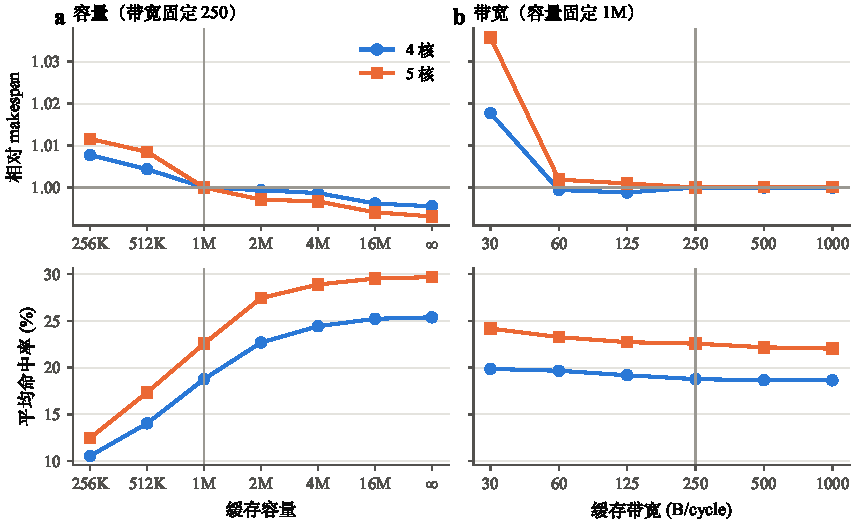
\includegraphics[width=\textwidth]{cache_sensitivity}
  \caption{缓存容量与带宽的敏感性（固定一批扫描阶段方案，只改缓存参数重评；竖线为官方配置）}
  \label{fig:sens}
\end{figure}

由此可以回答题目关于容量和带宽影响切图与调度的问题。在官方配置附近，这批方案对容量和带宽都不敏感，瓶颈不在缓存规格，而在读取的时机和分布。对切图而言，同一张量被越多的核心读取，缓存才越有用武之地，前提是这些读取在时间上错开；对调度而言，关键是让一个核心先把共享张量读进缓存，其他核心随后再读。这一结论来自固定的一批方案，不能直接推广到所有方案。

\label{sec:lockstep}并发缺失的一个典型形态是锁步读取。图~\ref{fig:lockstep} 是 \V{fig_lockstep_case} 在 \V{fig_lockstep_k} 核下一份历史方案的读取时间线（只画被多个核心读取的张量）。在官方配置下，同一张量被几个核心在几十个周期内先后发起读取，第一次读取还没完成，后面的全部未命中，一起挤在 DDR 上；每一轮都是如此，各核像齿轮一样同步推进，命中率只有 \V{fig_lockstep_hit250_pct}，Makespan 为 \V{fig_lockstep_ms250}。把缓存带宽从 250 降到 60 bytes/cycle，同一方案的命中率反而从 \V{fig_lockstep_hit250_pct} 升到 \V{fig_lockstep_hit60_pct}，Makespan 从 \V{fig_lockstep_ms250} 降到 \V{fig_lockstep_ms60}：更慢的缓存打乱了各核的相位，后读的核心晚到一步，恰好落在前一次读取完成之后。这说明在这类用例上，限制缓存收益的是式 \eqref{eq:hit} 中的时序条件，而不是容量条件。降低缓存带宽不是可行方案（配置固定），这个实验只用来确认机理。

\begin{figure}[H]
  \centering
  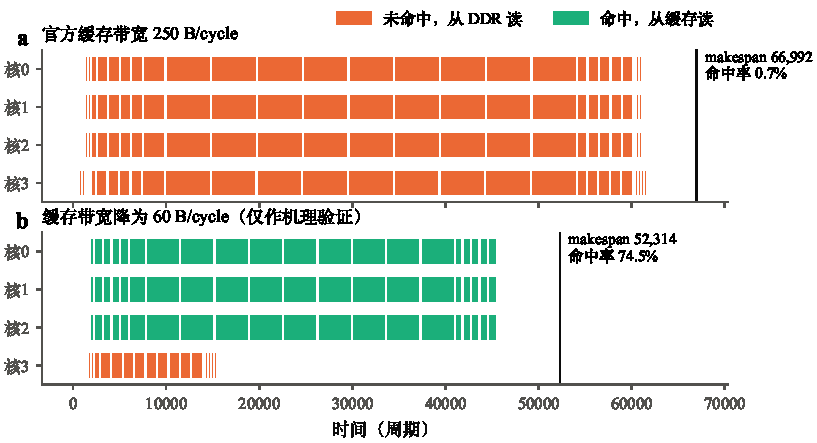
\includegraphics[width=\textwidth]{lockstep}
  \caption{锁步读取（\V{fig_lockstep_case}，\V{fig_lockstep_k} 核，同一份历史方案，只显示被多个核心读取的张量）。(a) 官方缓存带宽；(b) 缓存带宽降为 60 bytes/cycle，仅用于机理验证}
  \label{fig:lockstep}
\end{figure}

最后看两个典型用例。case\_090 在 5 核下的缓存加速比为 \V{cc_case_090_k5_best}，是全部用例中最高的：无 L2 的 Makespan 为 \V{cc_case_090_k5_noL2}，只读 Cache 下为 \V{cc_case_090_k5_cache}，命中率 \V{cc_case_090_k5_hit}。它的 4 核缺失分解中命中占 \V{cc_case_090_k4_share_hit_pct}，首次缺失只有 \V{cc_case_090_k4_share_compulsory_pct}，大量张量被多个核心重复读取，同时并发缺失仍有 \V{cc_case_090_k4_share_concurrent_pct}，若能进一步错开读取还有空间。图~\ref{fig:lockstep} 中的 case\_044 则是另一面：历史方案在问题三下的 Makespan 为 \V{fig_lockstep_ms250}，最终方案降到 \V{cc_case_044_k4_cache}（4 核），同方案缓存加速比为 \V{cc_case_044_k4_same}，命中率 \V{cc_case_044_k4_hit}，但并发缺失仍占 \V{cc_case_044_k4_share_concurrent_pct}，DDR 忙碌占比 \V{cc_case_044_k4_ddrbusy_pct}。最终方案主要靠更好的切图和分核缩短了时间，锁步读取并没有被消除。现有的构造与后处理只能间接改变读取时机，还不能主动控制它，这是本文在缓存利用上的边界。
